\documentclass[class=report, crop=false, 12pt,a4paper]{standalone}
\usepackage{enumitem}
\usepackage{multicol}
\usepackage{etoolbox}
\AtBeginEnvironment{quote}{\singlespacing\small}
\usepackage{setspace}
\onehalfspacing
\usepackage{graphicx}
\usepackage{float}
\usepackage{amsmath}
\usepackage{amssymb}
\usepackage{mathtools}
\usepackage{siunitx}
\sisetup{detect-all}
\begin{document}
\section{Momentum equation}
\begin{equation}
  \sum F_{sys} = \frac{\partial}{\partial t} \int_{CV} \underline{V} \rho d \forall + \int_{CS} \rho \underline{V} (\underline{V} \cdot \underline{n}) dA
\end{equation}
\subsection{Vane example:}
A horizontal jet of water exits a nozzle with a uniform speed of $V_1 = 3.048$ \si{\meter\per\second}, strikes a vane and is turned through an angle $\theta$. Determine the anchoring force needed to hold the vane stationary if gravity and visocus effects are negligible. 
\begin{figure}[h]
  \centering
  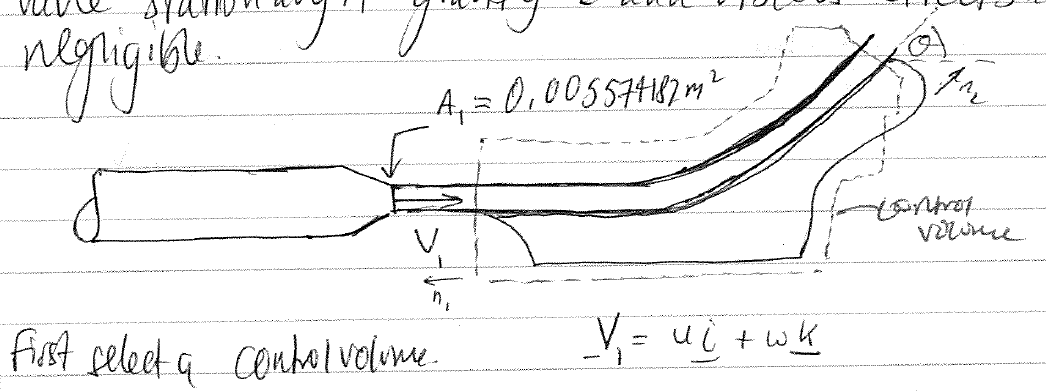
\includegraphics[width = 0.9\textwidth]{../img/Vanexample}
  \caption{Water flow through vane system.}
\end{figure}
The only portions of the control surfrace across which fluid flows are section 1 (the entrance) and section 2 (the exit). Hence, the momentum equation becomes in the x and z components.
\begin{align}
  \sum F_x &= \int_{inlet} u \rho (\underline{v} \cdot \underline{n}) dA + \int_{outlet} u \rho (\underline{V} \cdot \hat{n}) dA\\
  \sum F_x &= u_1 \rho (-V_1) A_1 + u_2 \rho (V_2) A_2\\
  \sum F_x &= u_2 \rho A_2 V_2 - i_1 \rho A_1 V_1
\end{align}
In the z direction:
\begin{align}
  \sum F_z &= \int_{inlet} w \rho (\underline{V}\cdot \hat{n}) dA + \int_{outlet} w \rho (\underline{V} \cdot {n}) dA\\
  \sum F_z &= w_2 \rho A_2 V_2 - w_1 \rho A_1 V_1
\end{align}
We know that at inlet $V_1$ there is no vertical component, hence $w_1 = 0$ and $u_1 = V_1$. At the outlet:
\begin{figure}
  \centering
  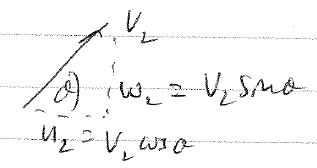
\includegraphics[width = 0.7\textwidth]{../img/Vanexample2}
  \caption{Velocity components at outlet.}
\end{figure}
Also lets find $V_1$ and $V_2$. From Bernoulli's equation (neglecting g, assuming incompressible and that $P_1 = P_2 = P_{atm}$), $V_1 = V_2$.
\begin{align}
  \therefore \sum F_z &= V_2 \sin{\theta} \rho A_2 V_2 = V_1^2 A_2 \sin{\theta} \rho \\
  \sum F_x &= V_2 \cos{\theta} \rho A_2 V_2 - V_1 \rho A_1 V_1\\
  \sum F_x &= V_1^2 A_2 \cos{\theta} \rho - V_1^2 \rho A_1 \\
  \sum F_x &= V_1^2 (A_2 \cos{\theta} \rho - \rho A_1)
\end{align}
\begin{figure}
  \centering
  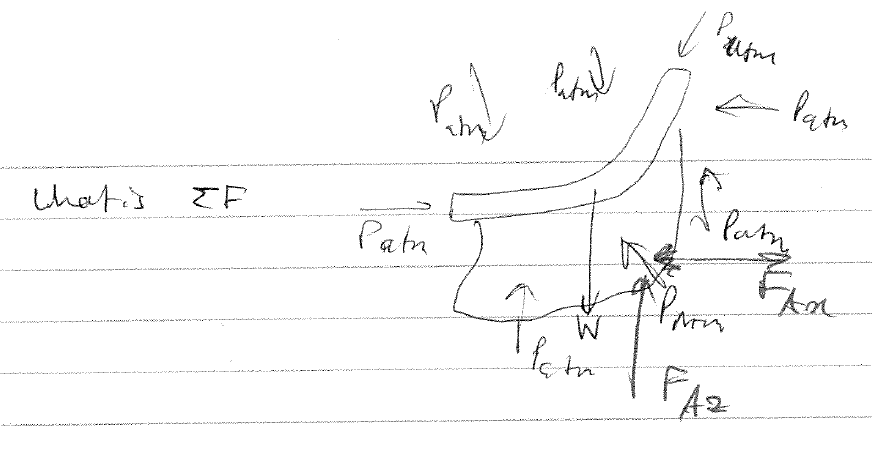
\includegraphics[width = 0.8\textwidth]{../img/Vanexample3}
  \caption{Forces acting on system.}
\end{figure}
Neglect $w$ and the net force due to $P_{atm} = 0$
\begin{align}
  \therefore \sum F_x &= F_{Ax}\\
  \sum F_z &= F_{Az}\\
  F_{Ax} &= V_1^2 A_2 \sin{\theta} \rho\\
  F_{Az} &= V_1^2 (A_z \cos{\theta} \rho - \rho A_1)
\end{align}
Also remember that,
\begin{align}
  \dot{m}_1 &= \dot{m}_2\\
  V_1 A_1 &= V_2 A_2 \textrm{ (incompressiblity)}\\
  V_1 = V_2 &\therefore A_1 = A_2\\
  \therefore F_{Ax} &= V_1^2 A_1 \sin{\theta} \rho \\
  F_{Az} = \rho V_1^2 (A_1 \cos{\theta} - A_1) &= \rho V_1^2 A_1 (\cos{\theta} - 1)
\end{align}
Plug in data to find $F_{Ax}$ and $F_{Az}$.
\end{document}